% Note: the document is written in LaTeX, hence the commands and macros in the manuscript.
% If you’re familiar with LaTeX, don’t hesitate to modify the commands, otherwise treat this document as a normal word document.

\documentclass[essd, manuscript]{copernicus}
\usepackage{hyperref}
\hypersetup{
    colorlinks = true,
    citecolor= blue
    }
\graphicspath{{../figures/paper/}}


\begin{document}

\title{Eutrophication climatologies for the European Seas}

\Author[1]{Charles}{Troupin}
\Author[1]{Alexander}{Barth}
\Author[1]{Jean-Marie}{Beckers}
\Author[2]{Karin}{Wesslander}
\Author[3]{Julie}{Gatti}
\Author[3]{Amandine}{Thomas}
\Author[3]{Erwann}{Quimpert}
\Author[5]{Jonas}{Koefoed Romer}
\Author[5]{Martin}{Mork Larsen}
\Author[6]{Luminita}{Buga}
\Author[6]{George}{Sarbu}
\Author[7]{Sissy}{Iona}
\Author[7]{Marilena}{Tsompanou}
\Author[8]{Ann Kristin}{Ostrem}
\Author[4]{Maria Eugenia}{Molina Jack}
\Author[4]{Marina}{Lipizer}
\Author[9]{Dick}{Schaap}
\Author[4]{Alessandra}{Giorgetti}


\affil[1]{University of Liège, FOCUS Research Unit, GeoHydrodynamics and Environment Research group (GHER), Allée du 6-Août, 17, 4000 Liège 1, Belgium} 
\affil[2]{Swedish Meteorological and Hydrological Institute Oceanographic Laboratory 2020-01-17 Dnr S/Gbg-2020-1 Address Sven Källfelts Gata 15 426 71 Västra Frölunda}
\affil[3]{French Institute for Ocean Science (IFREMER), 1625 Route de Sainte-Anne, 29280 Plouzané, France}
\affil[5]{Aarhus University, Department of Bioscience - Marine Diversity and Experimental Ecology, Frederiksborgvej 399 building 7411, B1.21, 4000 Roskilde, Denmark}
\affil[7]{Hellenic National Oceanographic Data Centre, 46,7 km Athens Sounio, Mavro Lithari P.O. BOX 712 19013 Anavissos, Attica, Greece}
\affil[6]{National Institute for Marine Research and Development “Grigore Antipa”. Location. B-dul Mamaia Nr. 300, Romina}
\affil[8]{Institute of Marine Research, P.O box 1870 Nordnes NO-5817 Bergen, Norway}
\affil[4]{Istituto Nazionale di Oceanografia e di Geofisica Sperimentale - OGS Borgo Grotta Gigante 42/C, 34010 Sgonico (TS), Italy}
\affil[9]{MARIS BV, Gildeweg 7 A BD Nootdorp, The Netherlands} %0000-0001-6562-068X

\correspondence{Charles Troupin (ctroupin@uliege.be)}

\runningtitle{Eutrophication climatologies for the European Seas}

\runningauthor{Troupin et al.}


\received{}
\pubdiscuss{} %% only important for two-stage journals
\revised{}
\accepted{}
\published{}

%% These dates will be inserted by Copernicus Publications during the typesetting process.


\firstpage{1}

\maketitle



\begin{abstract}
We present high-resolution, regional climatologies of eutrophication variables covering the European seas. The variables consist of ammonium, chlorophyll-a, dissolved inorganic nitrogen, dissolved oxygen, phosphate and silicate concentrations. The in situ observations are prepared and quality controlled following a standardised procedure. They are then interpolated using the Data-Interpolating Variational Analysis in n dimensions (DIVAnd) to create the climatologies. They are generated on a spatial domain covering all the Europeans seas, on 6 regional domains (Arctic Ocean, Northeast Atlantic Ocean, Baltic Sea, Black Sea, Mediterranean Sea and North Sea) as well as 4 coastal zones (Loire River, Gulf of Riga, Po River and Danube Delta).

The spatial resolution and the analysis parameters are adapted to each domain.
\end{abstract}


\introduction  %% \introduction[modified heading if necessary]

EMODnet (European Marine Observation and Data Network) is the in situ, marine data service of the European Commission Directorate-General Maritime Affairs and Fisheries \citep{MartinMiguez2019}. Initiated in 2009 as a pilot project, EMODnet is articulated according to the following features \citet{Shepherd2018}: 
\begin{enumerate}
\item The focus is on marine data; satellite data or fisheries survey are not considered; 
\item Multi-purpose data products, based on the raw data, are created and distributed; 
\item The data origin and ownership are preserved, both for the raw data and for the products; 
\item The observations are divided into thematic lots: bathymetry, biology, chemistry, geology, human activities, physics and seabed habitats. 
\end{enumerate} 

The EMODnet web portal has the objective of delivering marine data, products and metadata in a uniform and seamless way, thanks to common standards, procedures and vocabularies, following the
FAIR (Findable, Accessible, Interoperable, Re-usable) principles \citep {Wilkinson2016,Wilkinson2019}. Thanks to the always improving data access, a wider range of users can be reached, potentially leading to sustainable economic development, often referred to as the Blue Growth. 

One of the underlying principle of EMODnet can be summarised by the motto "\textit{Collect once, use many times}". Indeed, it is frequent that marine data are initially collected with a single purpose: this can a scientific project or a monitoring campaign. The combination of those observations with other sources of measurements or other parameters has the potential for the creation of new, added-value products that were not considered originally. Examples of such added-value products include:
\begin{enumerate}
\item The aggregated datasets: they consist of large ensembles of measurements obtained from various data providers; the measurements general undergo a suite of checks to ensure that their quality is good enough (depending on the final purpose).
\item The climatologies (or atlas): they consist of various gridded fields at different depth levels and for different time periods, obtained by interpolating the in situ observations on a regular grid.
\end{enumerate}

Both types of products are accompanied with metadata, which indicate how, when and by who the data were collected. For the climatologies, metadata also have to include information about all the individual data providers who contributed to the final products. 

The rest of the manuscript is organised as follows: first we describe the in situ observations used for the creation of the gridded products, since they already constitute a useful product; then we present the gridded technique, DIVAnd, applied to the observations; finally we describe the final product (climatologies). 


\section{In situ datasets\label{sec:insitu}}
%-------------------------------------------

EMODnet Chemistry is made up of 46 National Oceanographic Data Centres (NODCs) and focus on three main topics: eutrophication, marine contaminants and marine litter. The data management is governed by the SeaDataNet standards \citep{Schaap2010}, the Infrastructure for Spatial Information in Europe (INSPIRE) rules and the Open Geospatial Consortium (OGC) protocols. 

y involves around
100 institutes (nodes) from 35 countries 

Main goal = collection, harmonization and Quality Control of data gathered from national monitoring efforts and from research activities.
+ ensure Good Environmental Status \citep{Vinci2017}

 
The selected chemicals are relevant for the Marine Strategy Framework Directive (MSFD). 
Parameter names are based on the P01 Parameter Usage Vocabulary \url{https://vocab.seadatanet.org/p01-facet-search}
- Describe EMODnet Chemistry \citep{Giorgetti2018}

Two main types of data are considered: 
\begin{description}
\item[the profiles,] for which the primary variable is the depth;
\item[the time series:] for which the primary variable is the time (while the depth is generally fixed).
\end{description}
They are initially separated but then used together for the production of the climatologies. 

Unhomomegenety
- variables
- spatially
- tempoerally

these features make it necessary to have an indication of the error field

%
%\begin{figure}[t]
%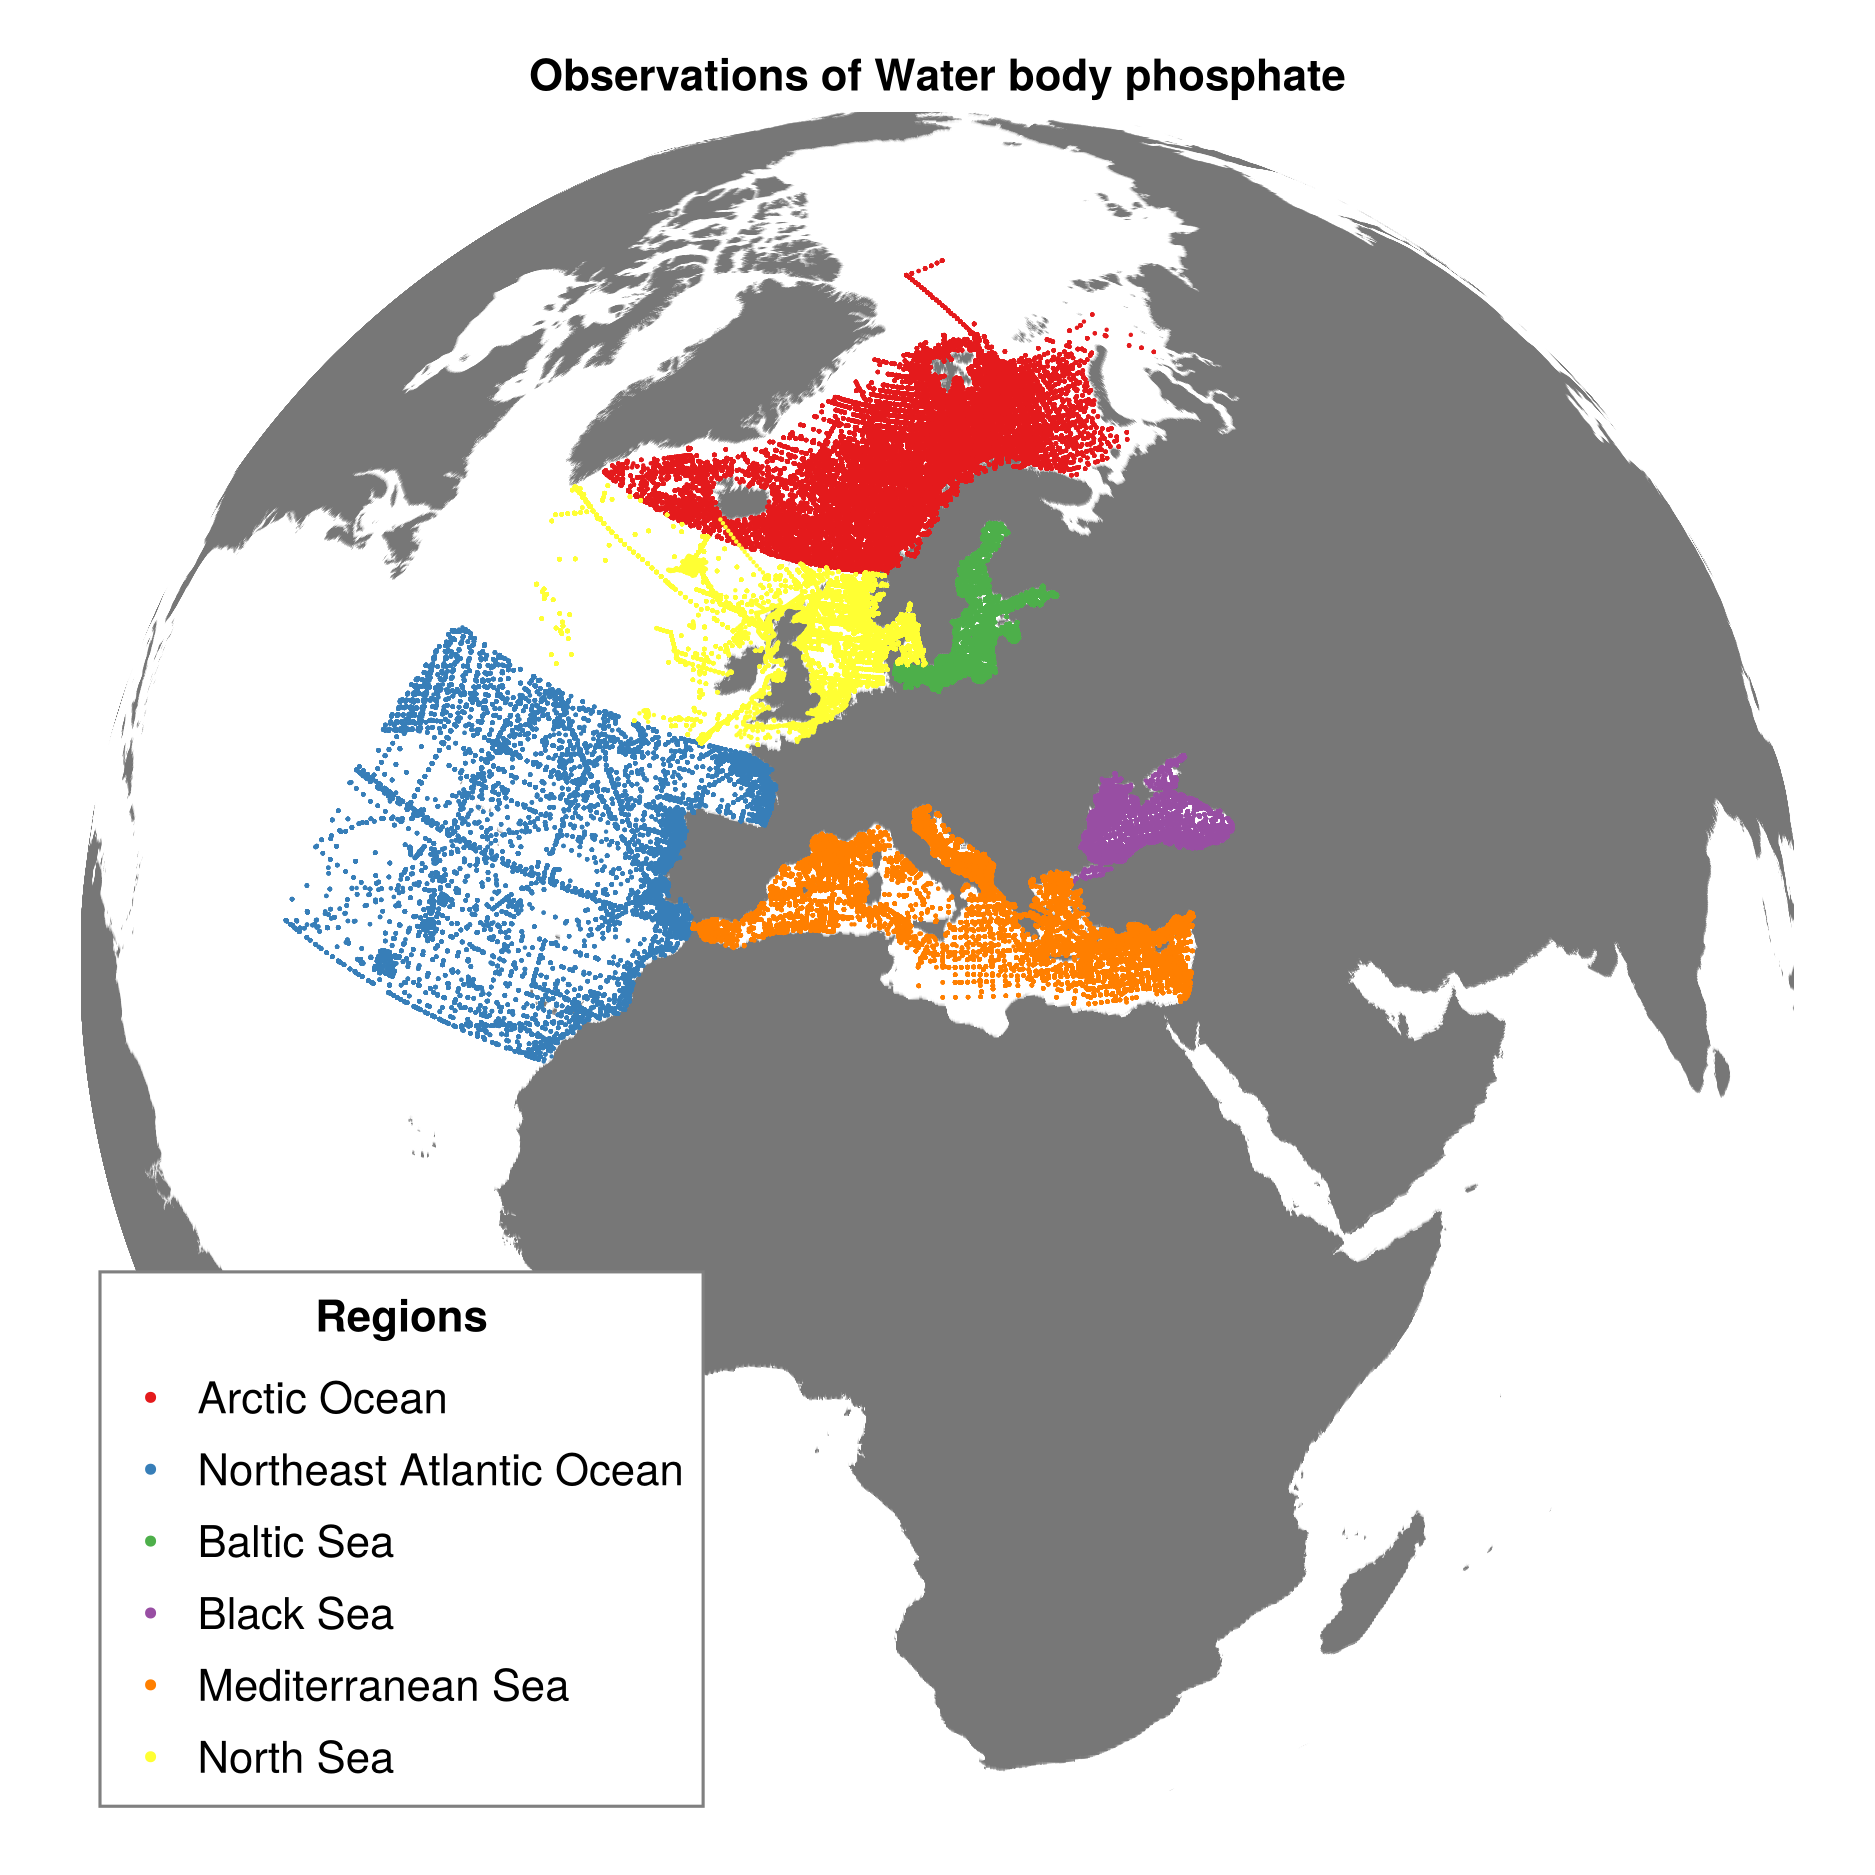
\includegraphics[width=8.3cm]{observations_Water_body_phosphate.png}
%\caption{Data locations corresponding to the phosphate concentration measurements.\label{fig:phosphatedata}}
%\end{figure}

\subsection{Metadata}

Common Data Index (CDI) Metadata profiles, based upon ISO 19115–19139 standards and supported by SeaDataNet Common Vocabularies

ne CDI (Common Data Index)
identifies a series of observations made at sea in the water column
(vertical profile) or in time (time series), with granularity defined by
data originator, sometimes in consultation with data managers. The
increase in total number of CDIs is shown i

\subsection{Variables}

 datasets on chemical substances
relevant for the assessment of Good Environmental Status (GES) ac-
cording to the MSFD Descriptors 5 (Eutrophication)



Eutrophication variables are those related to nutrients and their accumulation in the water column. In this work and for the sake of simplicity, the focus is placed on 6 of these variables, as summarised in Table~\ref{tab:variables}.

\begin{table}
\caption{List of variables with their corresponding standard name and units; used to produce EMODnet Chemistry products.\label{tab:variables}}
\begin{tabular}{llr}
\tophline
Variable 					& CF standard name														& Units		\\ 
\middlehline
Ammonium						& mole\_concentration\_of\_ammonium\_in\_sea\_water						& $\mu$mol/l	\\
Chlorophyll - a 				& mass\_concentration\_of\_chlorophyll\_a\_in\_sea\_water					& mg/m$^3$	\\
Dissolved inorganic nitrogen	& mole\_concentration\_of\_dissolved\_inorganic\_nitrogen\_in\_sea\_water & $\mu$mol/l	\\
Dissolved oxygen 			& mole\_concentration\_of\_dissolved\_molecular\_oxygen\_in\_sea\_water	& $\mu$mol/l	\\
Phosphate 					& moles\_of\_phosphate\_per\_unit\_mass\_in\_sea\_water					& $\mu$mol/l	\\
Silicate 					& mole\_concentration\_of\_silicate\_in\_sea\_water 						& $\mu$mol/l	\\
\bottomhline
\end{tabular}
\end{table}

\subsection{Domains}

The regional domains have been delimited in order to avoid overlay:
\begin{itemize}
\item The Mediterranean Sea and the Atlantic Ocean have their limit at the longitude of the Strait of Gibraltar.
\item The Sea of Marmara is assigned to the Mediterranean Sea region.
\item The North Sea and the NE Atlantic Ocean are separated by an imaginary line at 48°N, corresponding approximately to the latitude of Brittany (western France);
\item The Baltic Sea and the North Sea have their limit located in the Kattegat (between Denmark and Sweden).
\end{itemize}

The phosphate measurements corresponding to the 6~regional domains are shown in Fig.~\ref{fig:phosphatedata}, with the region boundaries defined in Tab.~\ref{tab:regions}. Along with the regional seas, 4 coastal regions are also defined. They are used for the creation of specific products near river mouth (see Sect.~\ref{sec:clim}). The phosphate distribution illustrates well the inherent lack of uniformity encountered with the measurements: most of the coastal zones are well sampled, with the exception of the southern part of the Mediterranean Sea east of Tunisia. The North Sea also exb 

\begin{table}
\caption{Spatial extend of the sea regions and the coastal areas.\label{tab:regions}}
\begin{tabular}{lrrrr}
\tophline
Region	 					& West		& East		& South 		& North 	 	\\ 
\middlehline	
Black Sea					& 26.5°E 	& 42°E		& 40°N		& 48°N	 	\\
Mediterranean Sea			& 6°W		& 36.375°E	& 30°N		& 46.375°N	\\
Baltic Sea					& 9.4°E		& 30.9°E		& 53°N		& 66°N		\\
North Sea 					& 5.4°W 		& 13°E		& 48°N		& 62°N		\\
Arctic Sea 					& 45°W 		& 70°E		& 62°N		& 83°N		\\
North-East Atlantic Ocean 	& 42°W		& 0° 		& 24°N		& 48°N		\\
\middlehline	
Danube delta					& 28.5°E		& 30.5°E		& 43.7°N 	& 45.6°N		\\
Gulf of Riga 				& 22.3°E 	& 25.0°E 	& 56.8°N 	& 58.4°N		\\
Loire estuary				& 4°W		& 1°W 		& 6.25°N		& 48°N		\\
Po river						& 12°E		& 14.0°E		& 44°N		& 46.0°N		\\
\bottomhline
\end{tabular}
\end{table}


		

\subsection{}

validation procedure to ensure the quality of the published datasets \citep{Barth2015,Lipizer2021}
involving the following checks
\begin{enumerate}
\item metadata completeness and dataset format; temporal and spatial (position, sampling depth, station bottom depth) information
must be present
\item harmonization of unit and parameter naming; this step is performed with ODV; a given variable is always expressed with the same units
\item quality flagging of data and metadata;
\item checks for clearly impossible data ranges.?
\end{enumerate} 


\subsection{File preparation}

The original files are provided in the form of ODV \citep[Ocean Data View,][]{SCHLITZER2002} collections. There are then converted to ODV netCDF, keeping the relevant metadata (i.e. those relative to the originators) in the exported files. Finally, the files are converted to ragged array netCDF using a script in Julia. The goal is to decrease the time needed to read the observations from the different regions: in the ODV netCDF files, the observations are organised by profile, and reading all of them means we have to loop over each profile. Meanwhile, for the creation of the gridded products, the information about the profile is not needed anymore and the data can be stored as vectors.

EDMO code and CDI \citep{Schaap2010}

With this format change, the files can be read in less than one minute (versus several hours for the ODV collections or ODV netCDF).

These operations were performed with ODV version 5.7.2 \citep{Schlitzer2024}.

\begin{table}
\begin{tabular}{lrr}
\tophline
Region			& Profiles		& Time series	\\
\middlehline
Arctic Ocean		& 145417			& 0				\\
Atlantic	 Ocean	& 389738			& 559			\\
Baltic Sea		& 211608			& 98				\\
Black Sea		& 75730			& 0				\\
Caribbean Sea	& 2863			& 91				\\
Mediterranean Sea & 253282		& 0				\\
North Sea		& 30804			& 134			\\
\bottomhline
\end{tabular}
\end{table}
 

\subsection{Spatial distribution}

The hexbin plot (Fig. ) provides another view on the data density. The regions with the highest coverage are located in the Baltic Sea and in the southern part of the North Sean while in general lower data densities are found at the edges of the global domain. The Mediterranean sea also exhibits an inhomogeneous data coverage. 

\begin{figure}[t]
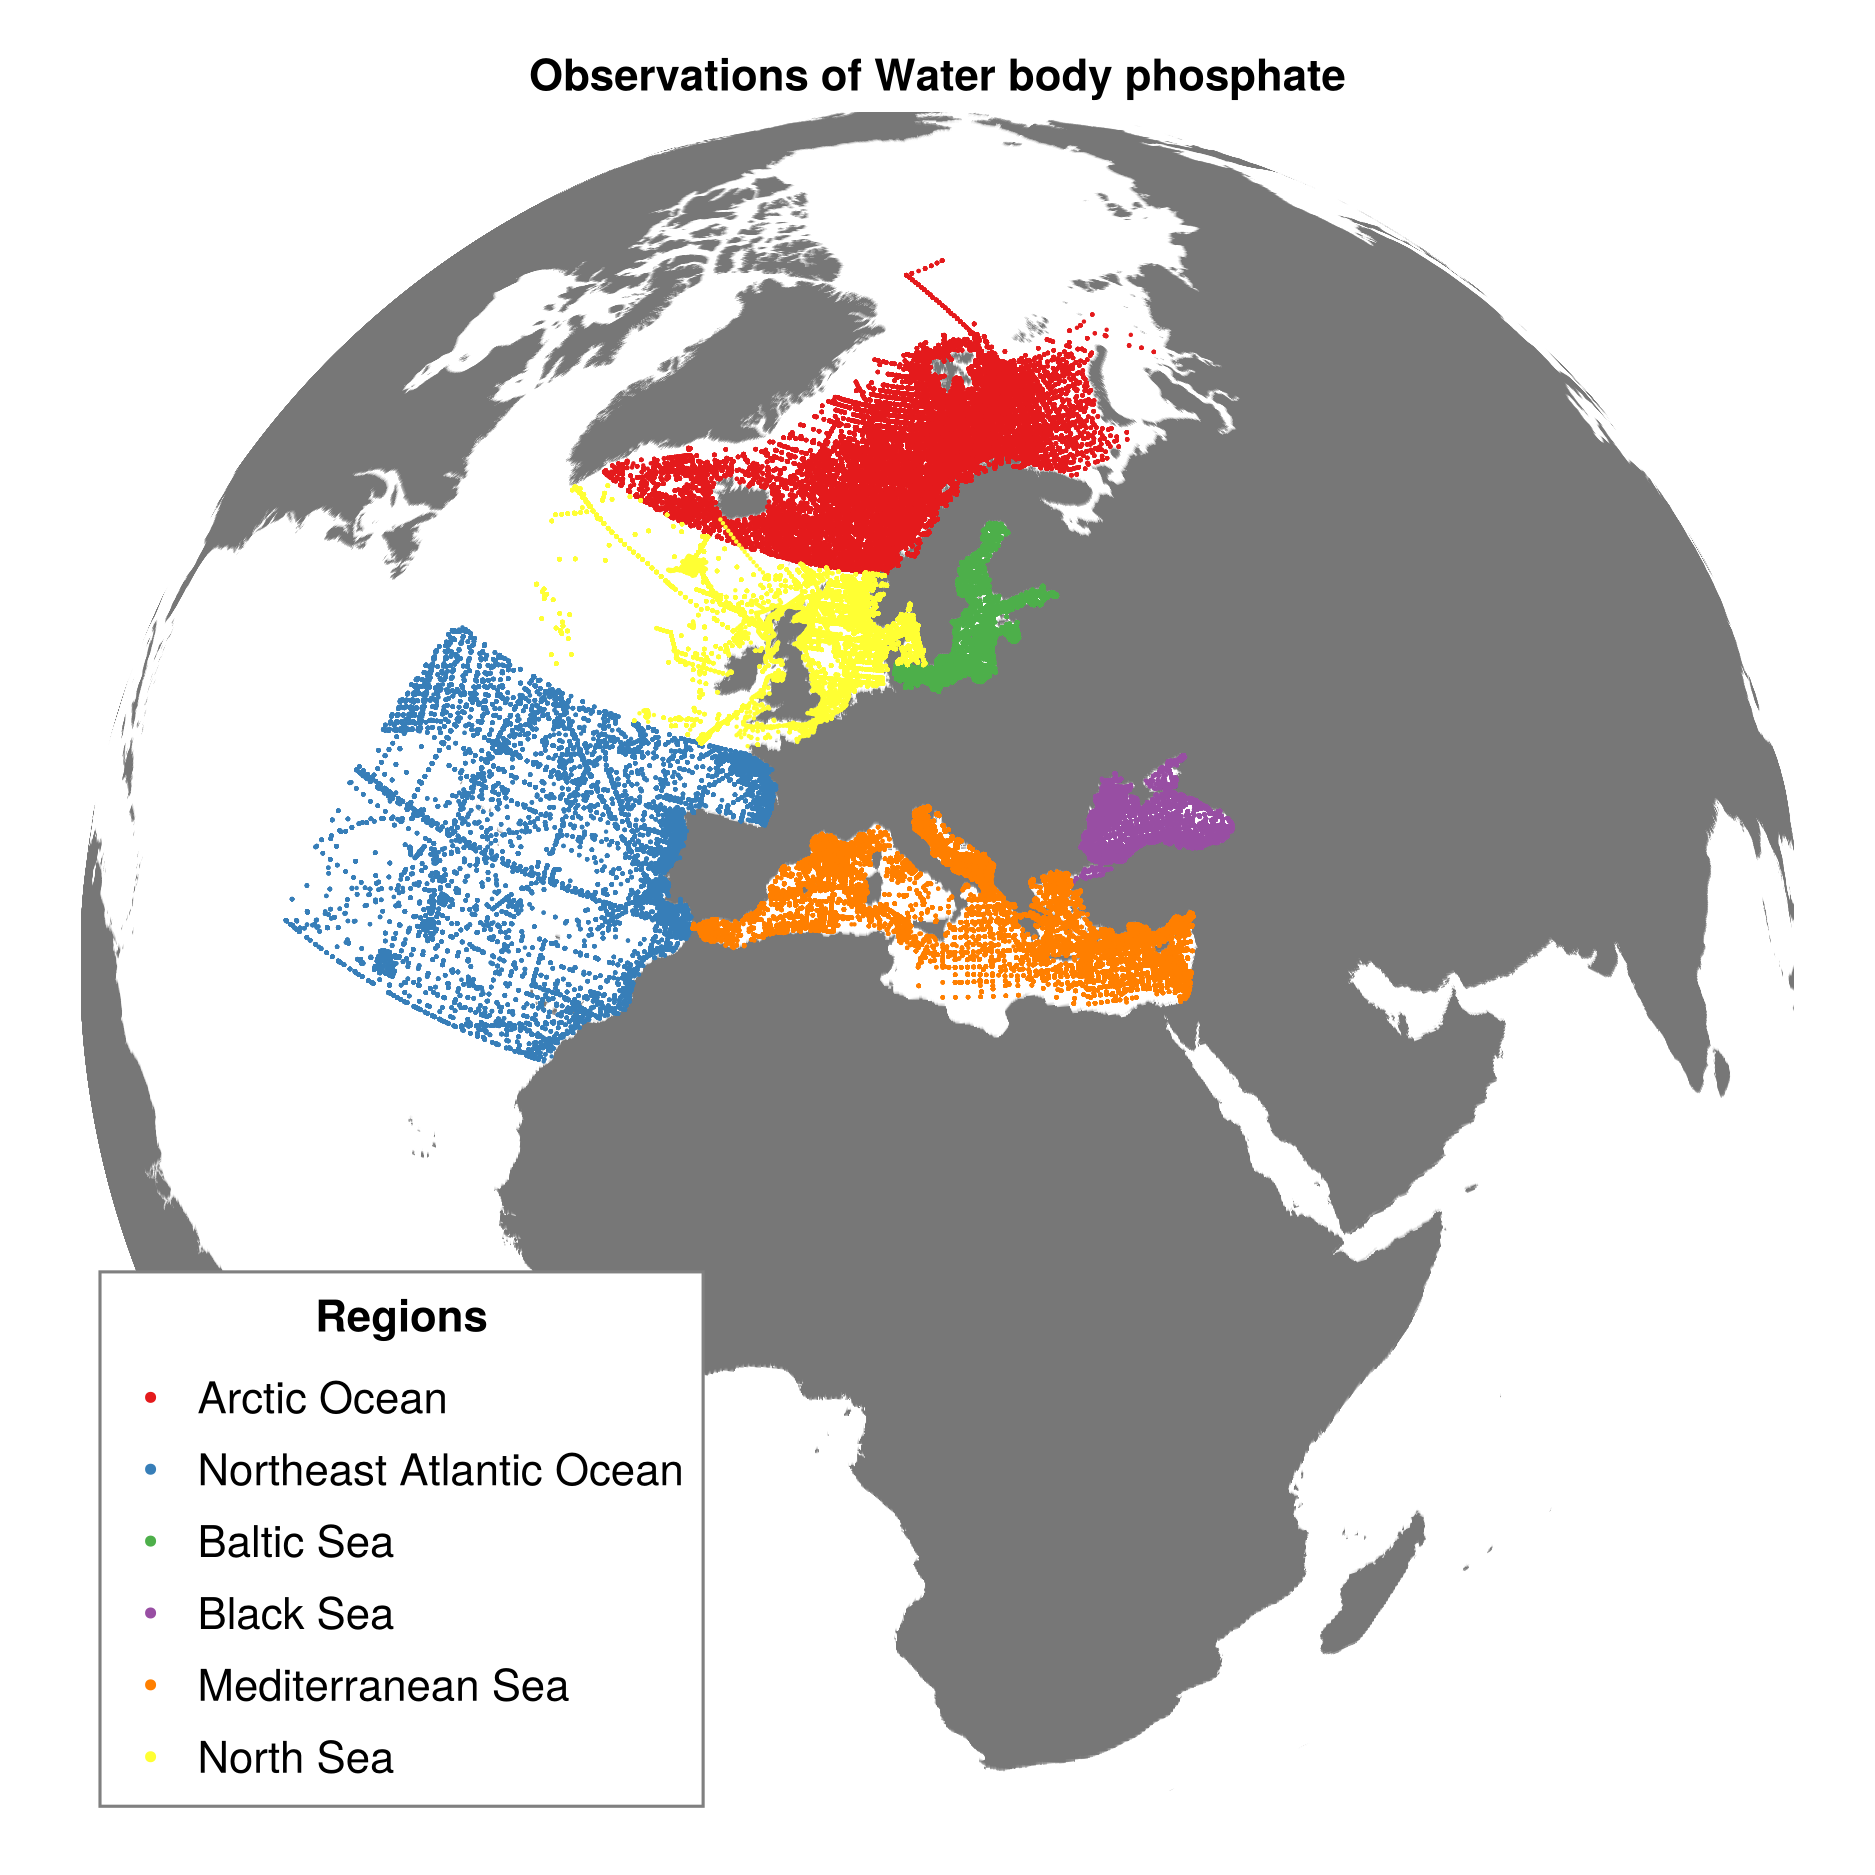
\includegraphics[width=8.3cm]{observations_Water_body_phosphate.png}
\caption{Locations of the phosphate concentration profiles.\label{fig:phosphatedata}}
\end{figure}

The panels of Fig. x also highlights the differences between the variables: for phosphate, silicate and oxygen, most of the domain is covered, whereas for ammonium, dissolved organic nitrogen and, to a lesser extent, chlorophyll, large subdomains are almost void of measurements. This will impact the quality of the interpolated field (Section …), which depends on the quality of the measurements and their availability.




\subsection{Temporal distribution}

\begin{figure*}[t]
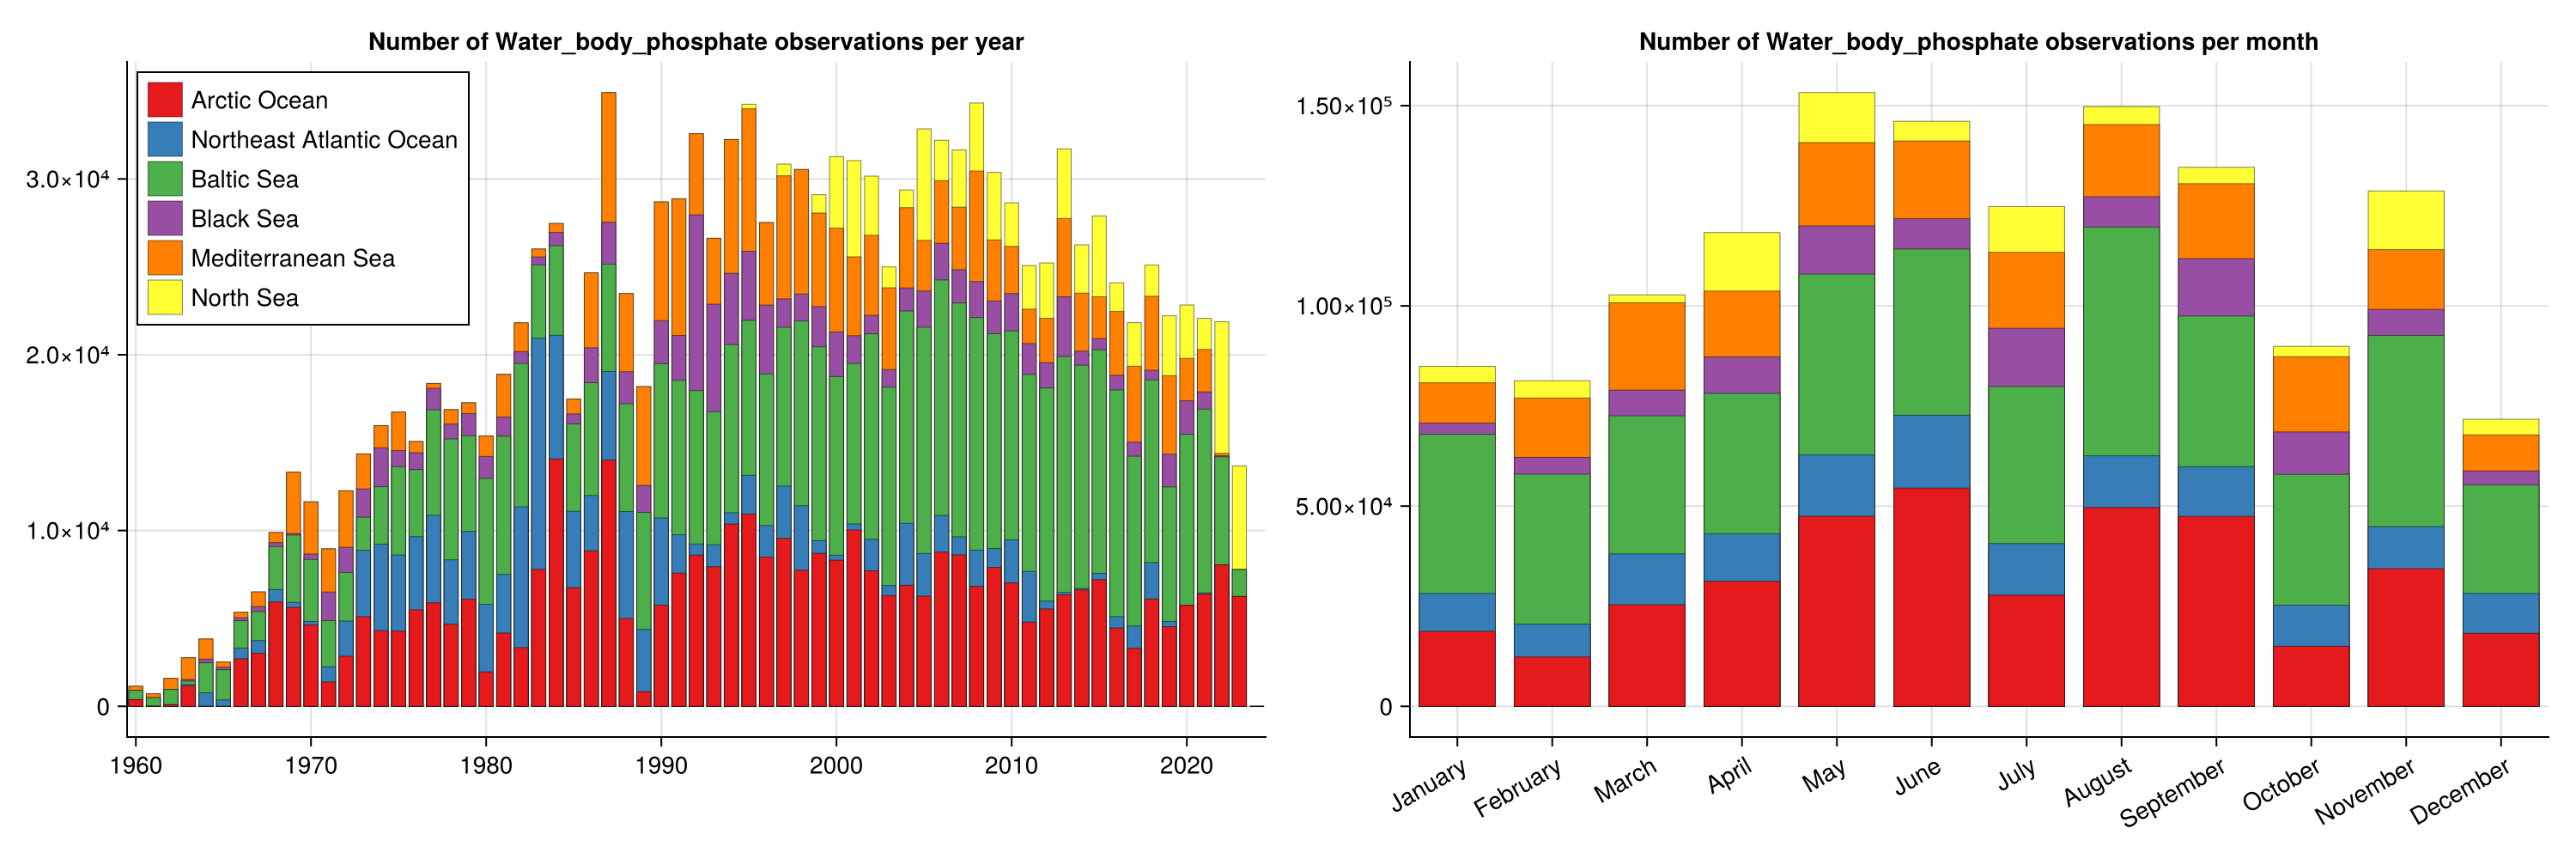
\includegraphics[width=12cm]{stacked_histogram_Water_body_phosphate.png}
\caption{Locations of the phosphate concentration profiles.\label{fig:phosphatedata}}
\end{figure*}


\subsection{Value distributions}

The value distribution (Fig. ) shows different patterns according to the variable considered. The dissolved oxygen concentration is the closest to a Gaussian. Ammonium, chlorophyll-a, nitrogen and silicate distributions are all characterised by a dominant number of measurements for small concentrations (close to zero) and few observations of high concentration. The case of phosphate seems to be a superposition of the two previous cases, where the lar


\subsection{File format}
The original data collections are provided as ODV (Ocean Data View) data collections \citep{Lowry2023}. Such collections are easily read then exported to another format using the ODV software tool {SCHLITZER2002}. In the present work we exported the collections to netCDF files, which are in turn are used as input files for the preparation of the climatologies (next Section). 
Along with the data (coordinates, time, depth and observed values), a set of metadata is assigned to each measurement. The complete list of metadata items is provided in the Appendix. Among them we find information about the instrument, the cruise and the institute that performed the measurements. 

\section{The interpolation method}

In this paper, we refer to \textit{gridding} as the process of computing the values of a variable (for instance: sea water temperature) on the nodes of a regular grid, based on observations of that variable at different locations and times.
The creation of gridded fields using sparse, in situ observations can be performed using different techniques. For the sake of simplicity, we will not review all of them but will insist on the distintion between two groups of tecniques:
\begin{enumerate}
\item The interpolation techniques: the field has to contain (or pass through) all the data points. For two-dimensional cases, an example of such a method is the bi-linear interpolation. Due to the different types of noise affecting the measurements in the ocean (instrumental, representativity, \ldots), such techniques are not the most suitable.
\item The approximation 
\end{enumerate}

The climatologies, consisting of a set of gridded fields for different depths and time periods, are produced by applying the Data Interpolating Variational Analysis in n dimensions (DIVAnd, see next Section) to the datasets presented in Section~\ref{sec:insitu}. Such gridded fields are frequently used in oceanography, for different purposes ranging from data visualisation to model initialisation or validation of measurements.  
While temperature and salinity (T and S) climatologies have been produced for various regions of the World Ocean using different interpolation techniques, climatologies for eutrophication-related variables are less frequent. The World Ocean Atlas (WOA) makes climatologies available for oxygen \citep[Dissolved Oxygen, Apparent Oxygen Utilization, and Oxygen Saturation][]{Garcia2024} and for dissolved inorganic nutrients \citep[phosphate, nitrate and nitrate+nitrite, silicate][]{Garcia2024b} at a resolution of 1° by 1° for the global ocean. The availability of measurements from the EMODnet Chemistry data collections makes it  possible to increase the spatial resolution in certain domains, hence the interest of the regional products presented in this paper.

% Check this → https://briochemc.github.io/WorldOceanAtlasTools.jl/stable/

\subsection{Method}

DIVAnd is an analysis method designed to generate fields on a curvilinear grid grid from a set of in situ measurements \citep{BARTH2014}. It is a new version of the DIVA tool \citep{TROUPIN2012,BECKERS2014} that was previously limited to 2 dimensions (usually longitude and latitude). With DIVAnd, it is now possible to perform the analysis on an arbitrary number of dimensions, typically the horizontal dimension (longitudes and latitudes), the vertical dimension (depth or pressure) and the time. With the previous version of  the DIVA tool, climatologies were obtained by stacking 2-dimensional layers computed for different depths and time periods. 
One of the main advantages of the method over widely used methods such as the Optimal Interpolation \citep[OI,][]{GANDIN1966,BRETHERTON1976} is that DIVAnd (and DIVA) naturally takes into account physical obstacles, typically the presence of land separating two bodies of water.  

DIVAnd is written in Julia \citep{Bezanson2017}, a fast, dynamically-type programming language, designed to ensure high-performance computation. While the previous code was written in Fortran, Julia ensures that high-resolution analysis using several millions of data points could be run in reasonable times, i.e. maximum a few days for the largest domain. This is necessary as usually to create a regional climatology, it is necessary to repeat the analysis several times in order to adapt the parameters and possibly remove suspect observations.

\subsection{Implementation}

\citep{TROUPIN2025}
A set of Jupyter-notebooks \citep[https://jupyter.org][]{KLUYVER2016} is
provided as guidelines explaining all the steps related to the creation of a climatology:
\begin{enumerate}
\item Data reading;
\item Creation of the land-sea mask based on the bathymetry;
\item Parameter optimisation;
\item Analysis;
\item Creation of figures.
\end{enumerate}

The GEBCO bathymetry (GEBCO 2021) was used with a resolution reduced by a factor 4 with respect to the original, was used for the creation of the land-sea mask
needed by DIVAnd (Fig.~\ref{fig:gebco_bathy_mask_domains3}).


%----------------------------------------------
\section{Gridded climatologies\label{sec:clim}}
%----------------------------------------------

\citep{BUGA2021}


\begin{figure*}[t]
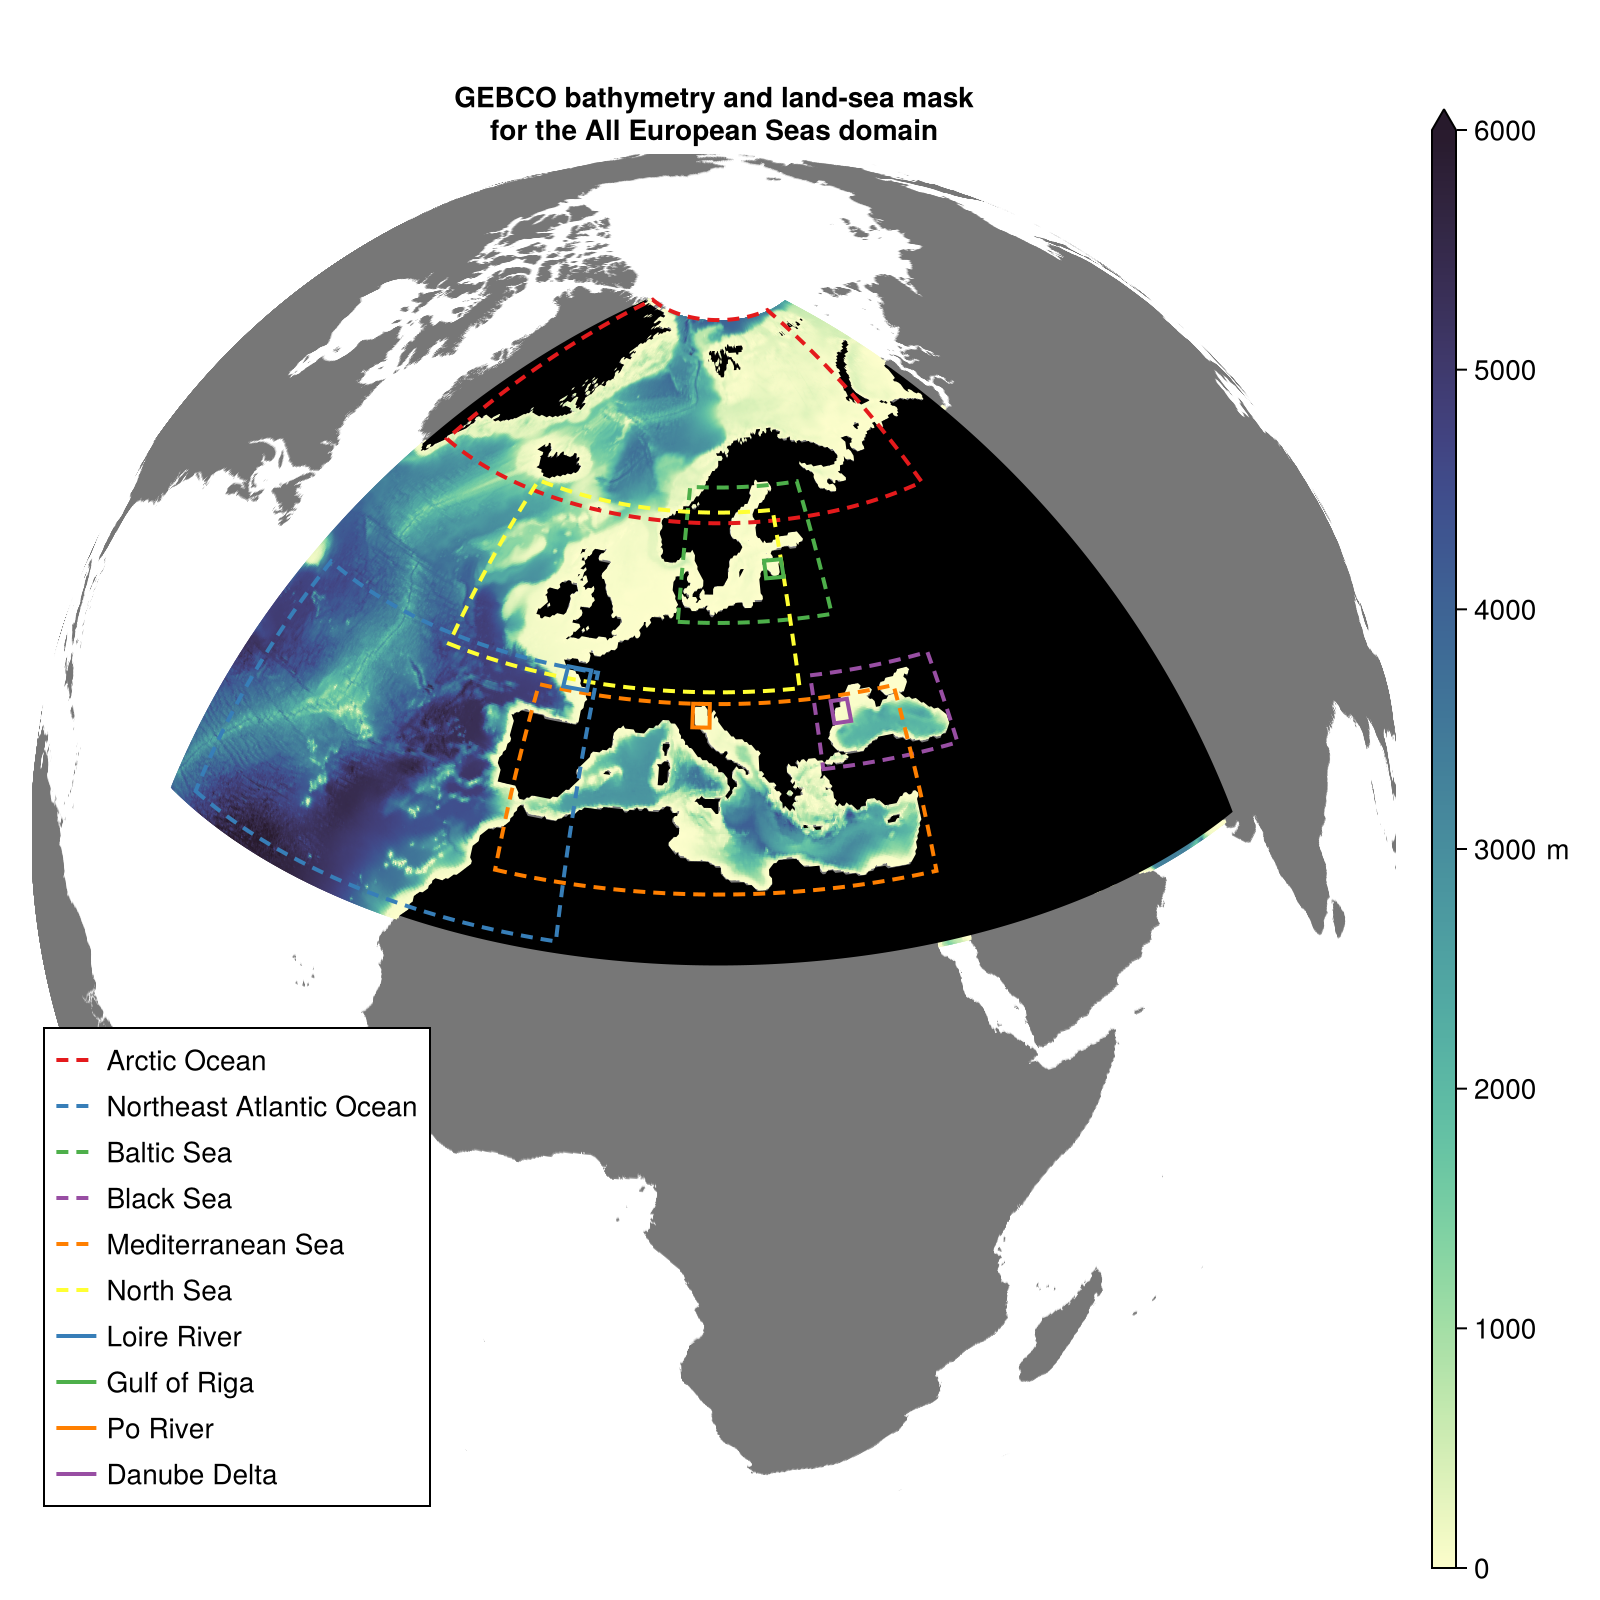
\includegraphics[width=12cm]{gebco_bathy_mask_domains3}
\caption{Bathymetry, surface land-sea mask and regional domains for the gridded products.\label{fig:gebco_bathy_mask_domains3}}
\end{figure*}

\subsection{Products}

Three types of climatologies were produced:
1. All European Seas – monthly maps on a domain covering all the regional seas
2. Sea region – at seasonal scale and for periods of 6 years, using a moving 6-year window
seasonal maps
3. Coastal area maps - at seasonal scale

EMODnet Chemistry Regional climatologies have been produced at seasonal scale and for periods of 6 years,
using a moving 6-year window. The season definitions used are defined specifically for each basin. 6-year
periods span from 1980-1985 until 2013-2018 (but highly depending on data availability for each sea/each
parameter/each season). 

\subsection{Product descriptions}

\subsubsection{File format}

The output of the analysis is a set of netCDF files storing the gridded fields generated by the analysis are written in netCDF \citep{Rew1990,Brown1993}, making use of the NCDatasets.jl library \citep{Barth2024}.

\subsubsection{Gridded variables}

The main variable stores the 4-dimension gridded field for each of the 6 selected variables. In addition, a relative error field informs about the confidence one can have in the results. It typically exhibit large values in region void of data, while the value are the lowest where the coverage is most dense. The error field is used to mask out the gridded field in regions where the error is considered to be too high. In practice, gridded fields masked using relative error threshold of 30\% and 50\% are calculated. The field masked with the 30\% error threshold is displayed as the principal layer in the Web Map Service (WMS). The motivation is to prevent users from interpreting the results where no data are available. 

Other variables containing the deepest values, masked with the same relative error thresholds, are also computed. 


% ADD plot of a given variable showing error field and masked field and deepest

\subsubsection{A posteriori quality control}

The initial data collections, presented in Sec.~\ref{sec:insitu}, underwent rigorous quality checks that ensure the final quality of the datasets. When performing analysis, it is also possible to detect suspicious data based on the residuals. The residual of a given data point is computed as the difference between the observed value and the analysed field at the location of the data point. In general, forcing the residuals to be small, i.e., to have an analysed field closed to the observations, does not guarantee good results: the field obtained will be noisy an not representative of a long-term mean state. Still, in an analysis performed with realistic parameters (here: correlation length and noise-to-signal ratio), large residuals might be the signal of either suspect data, or data not compatible with the climatology (HERE, NEED TO BETTER EXPLAIN).

The residuals for the pan-European gridded fields were provided to each regional leader. They were then asked to flag out suspect data, basing their decision on the values of the residuals. Finally, a new analysis was performed on a dataset in which the suspect observations were discarded. The locations of those discarded observations is presented in Fig.~\ref{fig:residuals}. 



\conclusions  %% \conclusions[modified heading if necessary]
TEXT

\codedataavailability{The DIVAnd source code is available at \url{https://github.com/gher-uliege/DIVAnd.jl} (\doi{10.5281/zenodo.1303229}, under the GNU General Public License v2.0. The Jupyter notebooks explaining how to create a climatology with DIVAnd are available at \url{https://github.com/gher-uliege/Diva-Workshops} (\doi{10.5281/zenodo.1248029}) under the MIT license. The merged data sets are provided at …, while the gridded fields are made available from the Sextant Catalog (\url{https://sextant.ifremer.fr/eng}). All the figures of this paper were produced with Makie and GeoMakie \citep{Danisch2021}.}





\authorcontribution{CT prepared the manuscript. ME and EQ coordinated the management of metadata (catalog and DOI). AB and CT: prepared the pan-European sea products; SI and MT: Mediterranean Sea. K.W. Baltic Sea; MML and JKR: North Sea; LB and GS: Black Sea; AKO: Arctic Sea; JG and NP: North Atlantic Ocean.} 

\competinginterests{The authors declare that there is no competing interest.}
\disclaimer{The data coverage obtained with the in situ measurements is heterogeneous, leading in higher uncertainties in the gridded field. The information contained in the gridded field believed to be trustworthy. However its accuracy and completeness cannot be guaranteed.  Whilst every effort has been made to ensure its reliability within the limits of present knowledge, no responsibility can be accepted by those involved in its compilation or publication for any consequential loss or damage arising from its use.
} 
\begin{acknowledgements}
The European Marine Observation and Data Network (EMODnet) is financed by the European Union under Regulation (EU) No 508/2014 of the European Parliament and of the Council of 15 May 2014 on the European Maritime and Fisheries Fund. Computational resources have been provided by the Consortium des Équipements de Calcul Intensif (CÉCI), funded by the Fonds de la Recherche Scientifique de Belgique (F.R.S.-FNRS) under Grant No. 2.5020.11 and by the Walloon Region. Part of the PHIDIAS project infrastructure (European Union’s Connecting Europe Facility under grant agreement No. INEA/CEF/ICT/ A2018/1810854) was used to run the pan-European Sea analysis. Aggregated data products are generated by EMODnet Chemistry under the support of DG MARE Call for Tenders EASME/EMFF/2016/006-lot4, EASME/2019/OP/0003-lot4. 
\end{acknowledgements}

\bibliography{emodnet.bib}
\bibliographystyle{copernicus.bst}


% The figure files should be labelled correctly with Arabic numerals (e.g. fig01.jpg, fig02.png).


%% ONE-COLUMN FIGURES

%%f
%\begin{figure}[t]
%\includegraphics[width=8.3cm]{FILE NAME}
%\caption{TEXT}
%\end{figure}
%
%%% TWO-COLUMN FIGURES
%
%%f
%\begin{figure*}[t]
%\includegraphics[width=12cm]{FILE NAME}
%\caption{TEXT}
%\end{figure*}
%
%
%%% TABLES
%%%
%%% The different columns must be seperated with a & command and should
%%% end with \\ to identify the column brake.
%
%%% ONE-COLUMN TABLE
%
%%t
%\begin{table}[t]
%\caption{TEXT}
%\begin{tabular}{column = lcr}
%\tophline
%
%\middlehline
%
%\bottomhline
%\end{tabular}
%\belowtable{} % Table Footnotes
%\end{table}
%
%%% TWO-COLUMN TABLE
%
%%t
%\begin{table*}[t]
%\caption{TEXT}
%\begin{tabular}{column = lcr}
%\tophline
%
%\middlehline
%
%\bottomhline
%\end{tabular}
%\belowtable{} % Table Footnotes
%\end{table*}
%
%%% LANDSCAPE TABLE
%
%%t
%\begin{sidewaystable*}[t]
%\caption{TEXT}
%\begin{tabular}{column = lcr}
%\tophline
%
%\middlehline
%
%\bottomhline
%\end{tabular}
%\belowtable{} % Table Footnotes
%\end{sidewaystable*}
%
%
%%% MATHEMATICAL EXPRESSIONS
%
%%% All papers typeset by Copernicus Publications follow the math typesetting regulations
%%% given by the IUPAC Green Book (IUPAC: Quantities, Units and Symbols in Physical Chemistry,
%%% 2nd Edn., Blackwell Science, available at: http://old.iupac.org/publications/books/gbook/green_book_2ed.pdf, 1993).
%%%
%%% Physical quantities/variables are typeset in italic font (t for time, T for Temperature)
%%% Indices which are not defined are typeset in italic font (x, y, z, a, b, c)
%%% Items/objects which are defined are typeset in roman font (Car A, Car B)
%%% Descriptions/specifications which are defined by itself are typeset in roman font (abs, rel, ref, tot, net, ice)
%%% Abbreviations from 2 letters are typeset in roman font (RH, LAI)
%%% Vectors are identified in bold italic font using \vec{x}
%%% Matrices are identified in bold roman font
%%% Multiplication signs are typeset using the LaTeX commands \times (for vector products, grids, and exponential notations) or \cdot
%%% The character * should not be applied as mutliplication sign
%
%
%%% PHYSICAL UNITS
%%%
%%% Please use \unit{} and apply the exponential notation


\end{document}

